\section{Work schedule and flow}\label{sec:workscheduleandflow}

In this section we deviate from talking about citizen science and Project Discovery and go over the work schedule and flow we followed during the project. We will discuss the methodology we decided to use to aid us during the project and how that influenced the project. We will go over the work schedule we put together and how we managed to follow that schedule. We will also show the burndown chart for the project as a whole and discuss all of the sprints that we finished while working on the project.

CCP Games graciously allowed us access to two work stations within their headquarters in Reykjavík, and placed us in an EVE development team with senior EVE developers who were available to us when we needed help with the project. They allowed us full access to the headquarters, along with the cafeteria with complementary lunch, which allowed us to stay in house and focus on the development of \emph{Project Discovery}.

\subsection{Methodology}
	For this project we utilized the Scrum methodology to help us document and organize the project and its progress. The appointed Scrum Master was Jóhann and the Product Owner was Hjalti. Pétur Örn Þórarinsson, a lead game designer at CCP, served as our Project Manager. Since the team only consisted of two people, the Scrum Master and Product Owner made up the the whole team. The project consisted of seven, two week long sprints, with the work divided so that the team could direct enough attention towards other courses, as well as work on the project.

	Daily Scrum meetings were held at CCP headquarters every work day. During the final three weeks of the project they took place at 11:30 AM, but they were held at various times of the day during the first 11 weeks, as the team wasn't always present throughout the day. We chose Scrum because it gave us good documentation on the team's progress and an indication of what we could achieve according to our velocity. With each iteration we could track what was going well and what needed improving. Scrum gave us the platform to review and improve on our process during each iteration.

\subsection{Initial plan}
	\subsubsection{Initial schedule}
		When we started the project, we estimated how much time we could afford to spend on the project, taking into account the workload from other courses. We ended up estimating that we had a total team capacity of 654 hours to spend during the entire project. A breakdown of how we scheduled those hours can be seen in table \ref{table:hours}. Work on the project was essentially split into two phases, the first one being the 12 week semester, from the 17th of August to November the 11th, in which other courses affected work on the project. The second one being the three week semester, from the 26th of November to December the 16th, where we could focus all our attention on the project. 
	  
	\begin{table}[H]
	  	\centering
		\addvbuffer[12pt 12pt]{\begin{tabular} {| l |  c | c |}
		\hline & Hjalti &  Jóhann\\
		\hline Total for 12 week semester & 162 hours & 192 hours \\
		\hline Total for 3 week semester & 150 hours & 150 hours \\
		\hline Total for the project & 312 hours & 342 hours \\
		\hline Total for the project combined & \multicolumn{2}{c |}{654 hours} \\ 
		\hline
		\end{tabular}}
		\caption{Breakdown of the initial schedule.}
		\label{table:hours}
	\end{table}

	\subsubsection{Initial stories}
		At the beginning of the project we, in collaboration with our project manager, populated a backlog of stories we felt we needed to implement. The backlog included 35 A stories, 9 B stories and 6 C stories, totaling 50 stories. Our goal was to at least finish all the A stories, any B or C stories would be a bonus. The A stories totaled 458 story points, the B stories totaled 106 story points and the C stories totaled 89 story points. Altogether the stories came to a total of 653 story points.

\subsection{Progress during the project}

	\subsubsection{Actual hours spent}
  We ended up spending some more time on the project than was scheduled, we spent 685 hours in total and went 31 hours over the plan to be specific. Most of the difference was during the 12 week term when we sometimes had crunch periods, for example getting features ready in time for EVE Vegas. A detailed view of the time we spent on the project can be seen in figure \ref{fig:total} where the x-axis represents each week during the project's time span and the y-axis represents the hours spent on the project each week. Overall we were both very pleased with each other's contribution and dedication to the project. 

		\begin{figure}[H]
      \centering
      \graphicspath{ {./graphics/} }
      \centerline{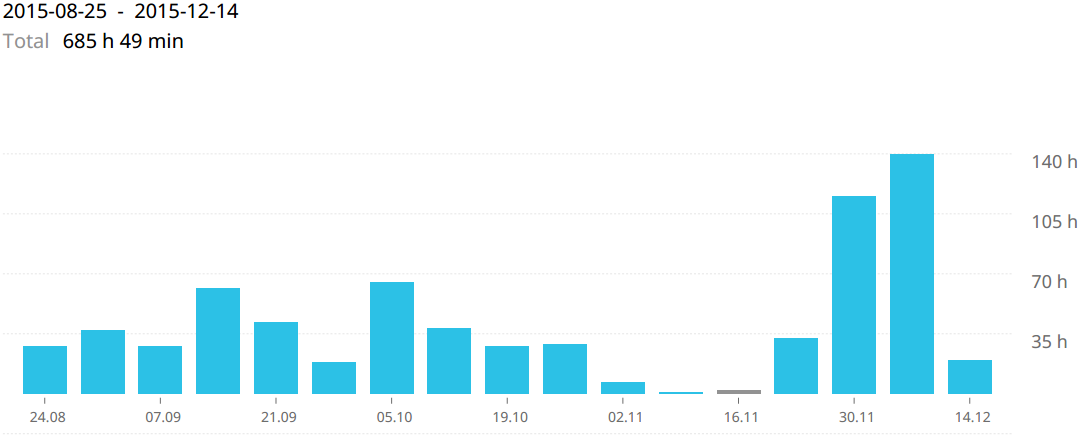
\includegraphics[scale=0.43]{total.png}}
      \caption{\label{fig:total} Breakdown of the hours we spent on the project.}
    \end{figure}
	
	\subsubsection{Actual stories}
		The stories we ended up implementing changed quite a lot from what we had planned. A lot of stories got added a during the project and a few got dropped because of changes to the project's focus. The main reason for this deviation from the plan was the user test we performed, it spawned a lot of new ideas and features that we hadn't even thought of before. At the end of the project we had 50 A stories, totaling 570 story points, 18 B stories with 251 story points and 5 C stories that totaled 64 story points. We decided to focus on finishing all the A stories, which we managed to do. Finishing those 570 story points gave us a velocity of 81.4 story points per sprint. The remaining B and C stories will hopefully be implemented in the near future, which we discuss in greater detail in section \ref{sec:futurework}.

	\subsubsection{Project burndown chart}
    The burndown chart for the entire project can be seen in figure \ref{fig:bdchart}. We estimated our velocity to be quite low for the first sprint since we figured it would take time to get acquainted with the project, the work environment and the tools we would need to work with. After that we estimated that our velocity would increase and average out to about 77 story points per sprint during the 12 week semester. For the last two sprints we estimated our velocity to be 114 story points per sprint as we would have more capacity during those sprints. 

    Our estimate was not far off the mark, although we sometimes did get behind schedule, we always managed to make up for it and we ultimately reached our goal. 
		
		\begin{figure}[H]
		  \centering
		  \graphicspath{ {./graphics/} }
		  \centerline{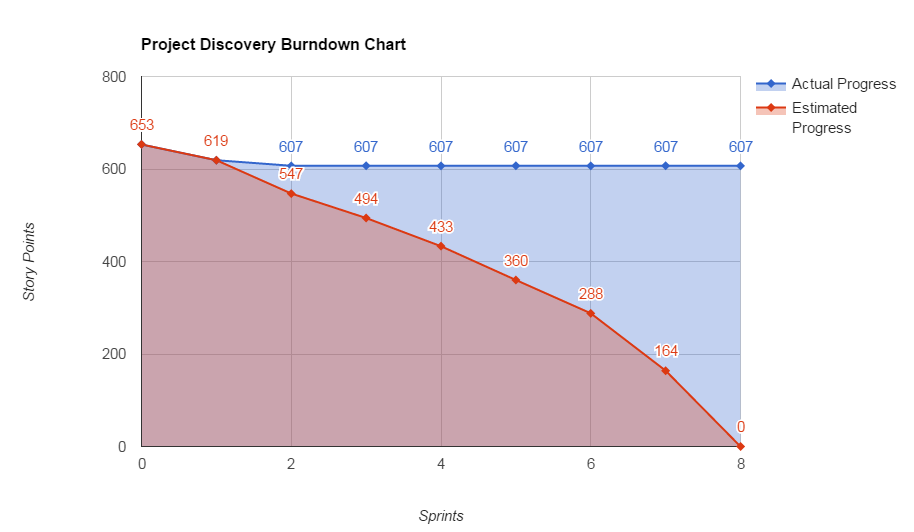
\includegraphics[scale=0.55]{bdchart.png}}
		  \caption{\label{fig:bdchart} Burndown chart for the whole project.}
		\end{figure}

	\subsubsection{Sprint summary}
  We did seven sprints in total and were able to refine our process and learn from our mistakes along the way. Early mistakes we made included underestimating stories which affected the consistency of our velocity, we also should have broken up larger stories to be able to finish them in a single sprint. The latter mistake resulted in us being behind schedule for sprints two and three but we managed to catch up in sprint four when we temporarily had more capacity and finished a lot of stories. In sprint five we again fell behind schedule as demands from other courses affected our capacity. We made up for it in sprints six and seven when we had a much greater capacity and no other courses to worry about. Those sprints went really well as by that time we had improved our process. 

\subsection{Schedule summary}
The initial plan changed quite a lot during the project, so the plan we set out with didn't really come to fruition. A lot of stories got added, we dropped a few stories and a lot of stories were set aside to be implemented in the future. We constantly adapted the backlog and the stories to the constantly evolving design of \emph{Project Discovery}. In the end we felt we met all our objectives and the plan worked out for us, as we delivered a game worthy of release to the \emph{EVE Online} test server. 

The Scrum methodology proved effective for the team. We were able to closely monitor our progress and make adjustments when necessary, it really helped to alert us when we were perhaps falling behind on our objectives.